% PS4 mathematical companion. Build with make in this directory.
% The slide order follows the assignment README; no reference results appear here.
% Worked numbers use the public checks' test trade (test/Fixtures.jl) at mid prices.
% The README and the starter docstrings cite five slides by number and title:
% "Building a structure from legs", "Profit at expiration", "Probability of
% profit by counting", "Return on capital and the margin rule", and "The four
% GBM models". The README also cites slide 15, "Exposure per 1% stock move".
% Update those citations if the slide order changes.
\documentclass[aspectratio=169,11pt]{beamer}
\usepackage{vnslides}
\newcommand{\ST}{S(T)}
\newcommand{\Prem}{\mathcal{P}}
\newcommand{\Pc}{\hat{P}_{\mathcal{C}}}
\newcommand{\one}{\mathbf{1}}
\newcommand{\POP}{\mathrm{POP}}
\newcommand{\IV}{\sigma_{\mathrm{IV}}}

% Profit diagrams: schematic two-panel PDFs in figs/, drawn in TikZ for the
% course. They carry no axis numbers; each slide note gives the test trade's.
\graphicspath{{figs/}}

\title{\texorpdfstring{{\vnheavy PS4}: Does Selling\\Options Pay?}{PS4: Does Selling Options Pay?}}
\subtitle{CHEME 4/5660 Cornell University | Mathematical Companion}
\author{Copyright Jeffrey Varner 2026. All Rights Reserved}
\begin{document}
\vntitlepage

\begin{frame}{Disclaimer and risks}
\textbf{Training only.} This assignment uses historical option quotes and
simplified trading assumptions for teaching. It provides no investment advice.

\vspace{1em}
\textbf{Selling options.} A short option collects its premium at entry but can
lose many times that amount. A short call with no protection has no limit on
its loss, and a broker can demand more money as the loss grows.

\vspace{1em}
\textbf{Simplifying assumptions.} One contract per leg, measured per share. Every
trade is held to expiration and settled at the stock's close that day, with no early
exercise or assignment. We omit commissions, dividends, taxes, and interest on
premiums. The quotes come from an indicative data feed.
\end{frame}

\begin{frame}{The central question}
Does selling option premium pay, and what does protection cost?
\vspace{0.2em}
\begin{itemize}\setlength{\itemsep}{0.15em}
\item \hilite{Study 1: the promise.} Build four structures from option legs.
Read each one's credit and its probability of profit under four price models.
\item \hilite{Study 2: the outcome.} Settle every trade at the stock's closing
price on the expiration date. Measure its profit, its return on capital, and
which model came closest to the win rate.
\item \hilite{Study 3: the conclusion.} Decide whether selling premium beat
the benchmarks and what protection cost, and see why every return is per trade.
\end{itemize}
Examples use the checks' test trade: entry price $S_0=100$, $D=30$ days to
expiration, and strikes (mid premiums, USD/share) of long put 80 (0.45), short
put 90 (1.25), ATM 100 (put 2.90, call 3.10), short call 110 (1.05), long call
120 (0.35).
\slidenote{Reading guide}{Both tracks do Studies 1–3. The put-side and call-side split on slide \pageref{fr:sides} is Advanced only.}
\end{frame}

\begin{frame}{Building a structure from legs}
A structure $\mathcal{C}$ is a set of option legs on one stock with one
expiration date. Each leg $i$ is a call or a put with strike $K_i$, number of
contracts $n_i=1$, premium $\Prem_i$, and orientation $\theta_i$, all per share:
\[
 \theta_i=\begin{cases}
 -1 & \text{short: you sell leg } i \text{, and } \Prem_i \text{ is its sell price},\\
 +1 & \text{long: you buy leg } i \text{, and } \Prem_i \text{ is its buy price}.
 \end{cases}
\]
The credit collected at entry is the premiums received minus those paid:
\[
 \text{credit}=-\sum_{i\in\mathcal{C}}\theta_i\,n_i\,\Prem_i .
\]
In code, each leg is one call to the course \texttt{build} function, with
\texttt{K}~$=K_i$, \texttt{premium}~$=\Prem_i$, \texttt{sense}~$=\theta_i$, and
\texttt{copy}~$=n_i=1$.
\slidenote{Also set}{\texttt{DTE}~$=D/365$, the years to expiration, and \texttt{IV}, the leg's implied volatility. The contract types require them; neither changes the profit at expiration.}
\end{frame}

\begin{frame}{The eight structures}
Each trade offers six legs. Their strikes sit around the entry price $S_0$, in
this order:
\[
 K_{\text{long put}}<K_{\text{short put}}<K_{\text{ATM}}\approx S_0
 <K_{\text{short call}}<K_{\text{long call}}.
\]
The at-the-money (ATM) call and put share the strike nearest $S_0$. The short
call and put are near 0.25 delta in absolute value, and the long call and put,
the wings, near 0.10.
\vspace{0.2em}
\begin{center}
\fontsize{9.5}{11.2}\selectfont
\begin{tabular}{@{}lll@{}}
\toprule
\vnmedium Structure & \vnmedium You sell ($\theta_i=-1$) & \vnmedium You buy ($\theta_i=+1$)\\
\midrule
Short straddle & ATM call, ATM put & nothing\\
Short strangle & short call, short put & nothing\\
Protected strangle & short call, short put & long call\\
Iron condor & short call, short put & long call, long put\\
\midrule
Short put \dimmed{(Advanced)} & short put & nothing\\
Short call \dimmed{(Advanced)} & short call & nothing\\
Put credit spread \dimmed{(Advanced)} & short put & long put\\
Call credit spread \dimmed{(Advanced)} & short call & long call\\
\bottomrule
\end{tabular}
\end{center}
\end{frame}

\begin{frame}{Profit at expiration}
At expiration, a call and a put with strike $K$ pay, per share:
\[
 V_c(K,\ST)=\bigl(\ST-K\bigr)^{+},\qquad V_p(K,\ST)=\bigl(K-\ST\bigr)^{+}.
\]
Here $\ST$ is the closing price on the expiration date and
$(x)^{+}=\max(x,0)$. With $V_i$ the payoff of leg $i$, $V_c$ or $V_p$, the
structure's profit is:
\[
 \Pc(\ST)=\sum_{i\in\mathcal{C}}\theta_i\,n_i\,
 \Bigl(\underbrace{V_i(K_i,\ST)}_{\text{payoff}}-\underbrace{\Prem_i}_{\text{premium}}\Bigr).
\]
The course \texttt{profit} function returns one row per share price: the
price, one column per leg, and the total $\Pc$ in the last column.

\vspace{0.4em}
Graded runs price every leg at its mid, $(\text{bid}+\text{ask})/2$; the
\textit{Fill prices and dollars} table compares bid/ask fills.
\slidenote{No interest}{PS4 omits \texttt{profit}'s optional accumulation factor $\mathcal{D}$ (default 1), which would grow premiums.}
\end{frame}

\begin{frame}{Profit diagrams: short legs only}\label{fr:diagrams-a}
The profit (black) is the structure's payoff $\sum_i\theta_i n_i V_i$ (blue) moved up by the credit.
\par\vspace{0.5em}
{\centering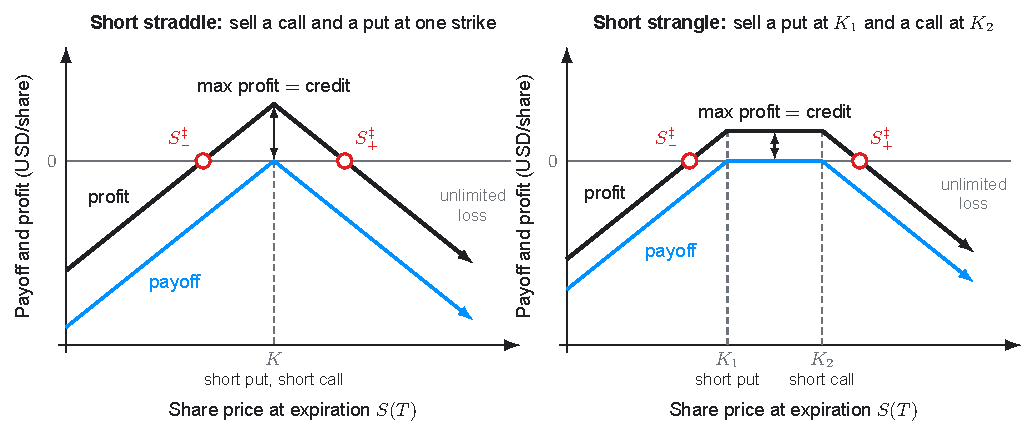
\includegraphics[width=0.74\textwidth]{Fig-Straddle-Strangle.pdf}\par}
\slidenote{Test trade}{Mid prices, USD/share; $K_1<K_2<\cdots$ label each diagram's own strikes. Straddle: credit 6.00, breakevens (zero profit) 94 and 106. Strangle: credit 2.30, breakevens 87.70 and 112.30.}
\end{frame}

\begin{frame}{Profit diagrams: adding long legs}\label{fr:diagrams-b}
Each long leg lowers the credit and caps the loss on its side.
\par\vspace{0.5em}
{\centering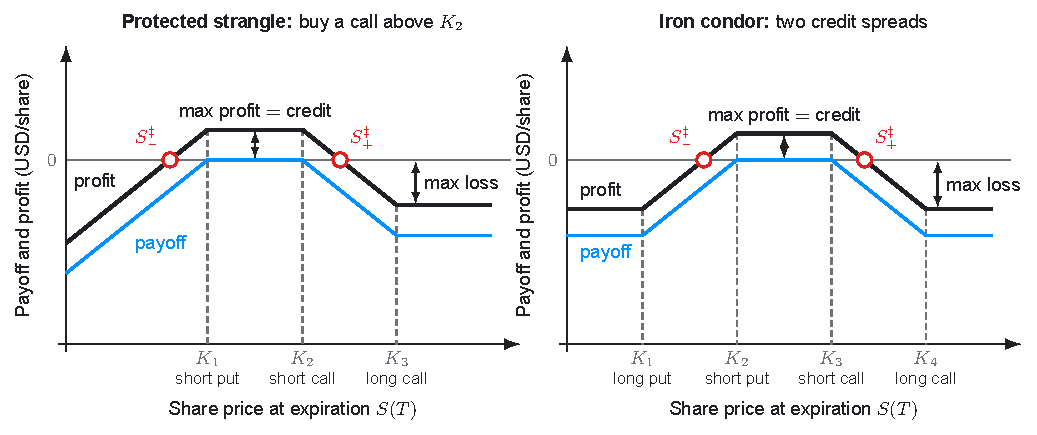
\includegraphics[width=0.76\textwidth]{Fig-Protected-Condor.pdf}\par}
\slidenote{Test trade}{Protected strangle: credit 1.95, breakevens 88.05 and 111.95, loss capped at 8.05 above 120 but not on a fall. Iron condor: credit 1.50, breakevens 88.50 and 111.50, loss capped at 8.50.}
\end{frame}

\begin{frame}{Return on capital and the margin rule}
Let $C$ be the capital set aside at entry, in USD/share. The return on capital
is the profit at expiration divided by the capital, $R=\Pc(\ST)/C$, a fraction
for one trade, not the lectures' annualized growth rate $g$.

\vspace{0.3em}
A naked short leg (no protection) with strike $K$ and premium $\Prem$ needs the
capital below. Here $S_0$ is the entry price, $m=0.20$ the margin rate, and
$f=0.10$ the floor:
\[
 C_{\text{call}}=\Prem+\max\bigl(mS_0-(K-S_0)^{+},\;fS_0\bigr),\qquad
 C_{\text{put}}=\Prem+\max\bigl(mS_0-(S_0-K)^{+},\;fK\bigr).
\]
\vspace{-0.4em}
\begin{itemize}\setlength{\itemsep}{0.2em}
\item \hilite{Straddle, strangle:} $\max(C_{\text{call}},C_{\text{put}})$; only one side can lose.
\item \hilite{Credit spread:} the strike width minus its own credit, its largest loss.
\item \hilite{Iron condor:} the wider of its two widths minus the total credit.
\item \hilite{Protected strangle:} the larger of $C_{\text{put}}$ and the call
credit spread's largest loss.
\end{itemize}
\slidenote{Test trade}{At mid prices, $C$ is 23.10 (straddle), 11.25 (short and protected strangles), and 8.50 (iron condor) USD/share.}
\end{frame}

\begin{frame}{Return on capital versus the share price}
Divide the profit and the capital by the entry price $S_0$:
\[
 R=\frac{\Pc(\ST)/S_0}{C/S_0}
  =\frac{\text{profit as a fraction of } S_0}{\text{capital as a fraction of } S_0}.
\]
The report's \textit{Capital (\% of share price)} column averages $C/S_0$. The
test trade's strangle sets aside 11.25\% of $S_0$, so a profit or loss of
1~USD/share, 1\% of $S_0$, is about 8.9\% of capital.
\vspace{0.5em}
\begin{itemize}\setlength{\itemsep}{0.45em}
\item \hilite{Every short leg protected.} A credit spread's lowest profit is
its credit minus its width, which is $-C$. The same holds for an iron condor,
so $R\geq-100\%$.
\item \hilite{A short leg without protection.} A short call can lose without
limit, and a short put up to its strike minus its premium. Then $R<-100\%$ is
possible, and a broker would demand more money. The protected strangle's put
is unprotected.
\end{itemize}
\end{frame}

\begin{frame}{Probability of profit by counting}
Each model on the next slide supplies $N=10{,}000$ simulated prices at expiration,
$S^{(1)}(T),\ldots,S^{(N)}(T)$. With the indicator $\one[\,\cdot\,]$, one when
its condition holds and zero otherwise, the probability of profit is the
fraction of prices with a positive total profit:
\[
 \widehat{\POP}=\frac{1}{N}\sum_{j=1}^{N}
 \one\Bigl[\Pc\bigl(S^{(j)}(T)\bigr)>0\Bigr].
\]
A simulated price with exactly zero profit does not count. Counting needs no
breakeven formula, so it works for any structure.

\vspace{0.6em}
A trade is \hilite{won} when its profit at the one actual closing price is
positive, $\Pc(\ST)>0$.
\slidenote{Precision}{With $N=10{,}000$, the standard error $\sqrt{\widehat{\POP}(1-\widehat{\POP})/N}$ is at most 0.5 percentage points per trade. A win rate over 174 trades has a standard error of up to 3.8 points.}
\end{frame}

\begin{frame}{The four GBM models}
Each model is a geometric Brownian motion with drift $\mu$ and
volatility $\sigma$ per year. The course \texttt{sample} function steps one
day, $\Delta t=1/365$ year, from entry at price $S_0$ to expiration at $T=D/365$:
\[
 S_{t_j}=S_{t_{j-1}}\exp\Bigl[\bigl(\mu-\tfrac{\sigma^2}{2}\bigr)\Delta t
 +\sigma\sqrt{\Delta t}\,Z_j\Bigr],\qquad t_j=j\,\Delta t,\quad Z_j\sim\mathcal{N}(0,1).
\]
The models differ only in $\mu$ and $\sigma$. The risk-free rate is
$r=0.0376$ per year, and $\IV$ is the mean of the ATM call's and put's
implied volatilities at entry:
\vspace{0.2em}
\begin{center}
\fontsize{9.5}{11.5}\selectfont
\begin{tabular}{@{}lll@{}}
\toprule
\vnmedium Report column & \vnmedium Drift $\mu$ & \vnmedium Volatility $\sigma$\\
\midrule
Model POP: market (r, IV) & $r$ & $\IV$\\
Model POP: historical drift, IV & $\hat\mu$ (slide \pageref{fr:hist}) & $\IV$\\
Model POP: r, historical vol & $r$ & $\hat\sigma$ (slide \pageref{fr:hist})\\
Model POP: historical drift and vol & $\hat\mu$ & $\hat\sigma$\\
\bottomrule
\end{tabular}
\end{center}
\slidenote{Same draws}{The four models of a trade reuse the same $Z_j$, so their probabilities differ because of $\mu$ and $\sigma$, not chance.}
\end{frame}

\begin{frame}{Historical drift and volatility}\label{fr:hist}
From the last 253 daily closes before the entry date, $c_0,\ldots,c_{252}$, with
log changes $\ell_k=\ln(c_k/c_{k-1})$ and their mean $\bar\ell$, the annualized
log growth rate $\hat g$ and volatility $\hat\sigma$ are:
\[
 \hat g=252\,\bar\ell,\qquad
 \hat\sigma=\sqrt{252}\,\sqrt{\frac{1}{251}\sum_{k=1}^{252}\bigl(\ell_k-\bar\ell\bigr)^2}.
\]
The course \texttt{sample} grows the log price at $\mu-\sigma^2/2$, so the
historical drift that gives log growth $\hat g$ is:
\[
 \hat\mu=\hat g+\frac{\hat\sigma^2}{2},
 \qquad\text{so that}\qquad
 \hat\mu-\frac{\hat\sigma^2}{2}=\hat g.
\]
The historical drift, IV model changes only the market model's drift, to
$\hat\mu$; its log price grows at $\hat\mu-\IV^2/2$, equal to $\hat g$ only if
$\IV=\hat\sigma$.
\slidenote{Two calendars}{Daily changes are annualized with 252 trading days, $T$ with 365 calendar days. They agree: about 21 trading days span 30 calendar days.}
\end{frame}

\begin{frame}{Win rate, average return, and probability of profit}
For the $n$ trades of one structure, let $P_k$ be trade $k$'s profit at
expiration, $R_k$ its return on capital, and $\POP_k$ a model's probability of
profit. Three averages answer three questions:
\[
 \underbrace{W=\frac1n\sum_{k=1}^{n}\one[P_k>0]}_{\text{how often it won}},\qquad
 \underbrace{\bar R=\frac1n\sum_{k=1}^{n}R_k}_{\text{what it earned}},\qquad
 \underbrace{\overline{\POP}=\frac1n\sum_{k=1}^{n}\POP_k}_{\text{what a model promised}}.
\]
Split the trades into wins and the others, with average returns
$\bar R_{\text{win}}$ and $\bar R_{\text{loss}}\leq0$:
\[
 \bar R=W\,\bar R_{\text{win}}+(1-W)\,\bar R_{\text{loss}}.
\]
So $\bar R<0$ whenever $(1-W)\,\lvert\bar R_{\text{loss}}\rvert>W\,\bar R_{\text{win}}$,
however high $W$ is. A few large losses move the mean far more than the
median, which the report also lists.
\slidenote{Equal weights}{$\bar R$ is the return of putting the same dollar capital into every trade.}
\end{frame}

\begin{frame}{Exposure per 1\% stock move}
\setlength{\abovedisplayskip}{4pt}\setlength{\belowdisplayskip}{4pt}%
A leg's delta $\Delta_i$, from the entry quotes, is its price change per
$+1$~USD/share rise in the share price. The structure's delta adds the legs:
\[
 \Delta_{\mathcal{C}}=\sum_{i\in\mathcal{C}}\theta_i\,n_i\,\Delta_i .
\]
A 1\% rise moves the price by $0.01\,S_0$ and the structure's value by about
$\Delta_{\mathcal{C}}\times0.01\,S_0$. The report's \emph{Change in value per 1\%
stock rise} divides this by the capital:
\[
 E=\frac{\Delta_{\mathcal{C}}\times0.01\,S_0}{C}.
\]
A share bought outright has $E=1\%$; $E=2\%$ is twofold leverage. The test trade's short put ($\Delta_i=-0.25$,
$\theta_i=-1$) has $E=0.25\times1.00/11.25\approx2.2\%$.
\slidenote{First order}{An $x$\% move changes the value by about $x\,E$ of capital. Deltas change as the stock moves: a short straddle starts near $E=0$ yet loses on a large move either way.}
\end{frame}

\begin{frame}{Why annualizing a per-trade return misleads}
A trade lasts $D\approx30$ calendar days, so a year holds about
$365/D\approx12$ trades. Two common ways to turn a per-trade return $R$ into a
yearly figure are:
\[
 \underbrace{\frac{365}{D}\,R}_{\text{simple}}
 \qquad\text{and}\qquad
 \underbrace{(1+R)^{365/D}-1}_{\text{compounded}}.
\]
Both assume every month earns the same $R$, which causes three problems:
\begin{itemize}\setlength{\itemsep}{0.3em}
\item the next twelve trades need not win and lose as the sampled trades did;
\item an average over a limited sample with rare large losses is uncertain, and
multiplying it by 12 multiplies that uncertainty by 12;
\item compounding reinvests all capital, which needs $1+R>0$ every month.
\end{itemize}
The test trade's strangle earns $R=+20.4\%$ at an unchanged price;
multiplied by 12, about one trade a month, that gives about $+245\%$. A close at 130~USD/share gives
$R=-157.3\%$, so $1+R<0$ and compounding breaks down.
\end{frame}

\begin{frame}{Advanced: the put side and the call side}\label{fr:sides}
The iron condor is the two credit spreads below. Their profits add,
$\Pc(\ST)=\hat P_{\text{put side}}(\ST)+\hat P_{\text{call side}}(\ST)$, but their
returns on capital do not: each side has its own capital.
\par\vspace{0.5em}
{\centering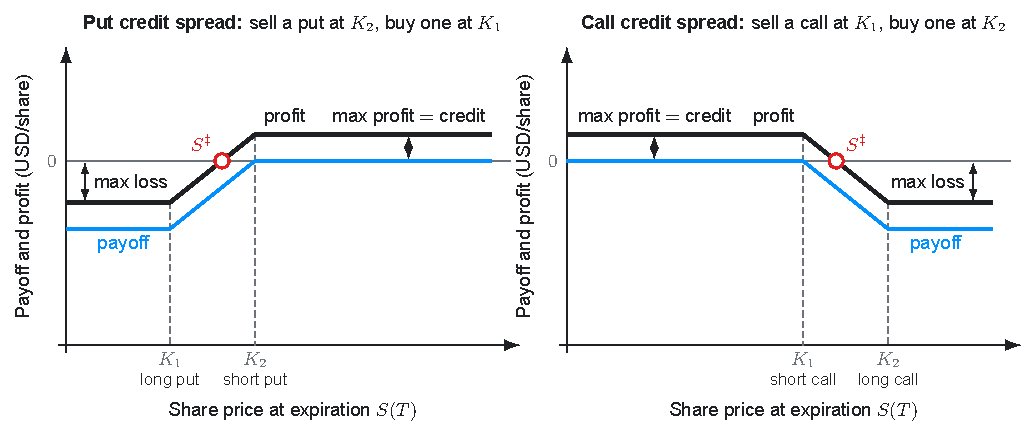
\includegraphics[width=0.6\textwidth]{Fig-Credit-Spreads.pdf}\par}
\slidenote{Also split}{The short strangle (short put, short call) and the protected strangle (short put, call credit spread). Compare the sides by average profit.}
\end{frame}

\begin{frame}{Summary}
PS4 builds option-selling structures from legs, compares what price models
promised with what happened at expiration, and measures each profit against
the capital a broker would require.

\vspace{0.6em}
\textbf{Key takeaways}
\begin{itemize}\setlength{\itemsep}{0.5em}
\item A structure's profit at expiration is the sum of its legs' profits. A
long leg costs part of the credit and caps the loss on its side.
\item The model probability of profit, the win rate, and the average return
on capital answer different questions. A high win rate alone does not give a
positive average.
\item Return on capital and exposure are measured against the capital, a
fraction of the share price, so they swing far more than the stock's own return.
\end{itemize}
\vspace{0.6em}
Use these measures, per trade and never per year, to answer the central
question.
\end{frame}
\end{document}
